\chapter{Observational Analysis}
\label{ch_4}


% ------------------------------------------------------------------
\section{Making Polarization Maps}
\label{sec: chap4_polarization_vectors}
% ------------------------------------------------------------------
The polarization morphology of a disk is represented by polarization vectors calculated from \SQ and $U$, which define the polarization angle (Equation \ref{eq: PA}). From these morphologies, the dominant polarization mechanism can be inferred, as different mechanisms produce different polarization patterns (see Chapter \ref{sec: intro_polarization_mechanisms}). By comparing the polarization morphologies at multiple wavelengths, we can examine how the dominant polarization mechanism changes with optical depth. We first calculated the polarization vector and then created models to fit the observed morphologies and determine the dominant mechanisms. 
% ------------------------------------------------------------------



% ------------------------------------------------------------------



\subsection{Polarization Vector Sampling}

%\later{Might not be needed but okay to include. Will decide later.}

The \SI maps produced using \texttt{tclean} have a pixel scale that oversamples the synthesized beam to improve image reconstruction \citep{Brogan}. Because of these small pixels, plotting a polarization vector at each pixel would oversample the polarization morphology. Instead, vectors are plotted with a spacing of approximately half of the synthesized beam size, following the Nyquist-Shannon sampling theorem \citep{Shannon}. 

The effective beam size was calculated using:
\begin{equation}
    \text{Beam Size =} \sqrt{\text{BMIN} \cdot \text{BMAJ}},
    \label{eq: beam_size}
\end{equation}
\noindent where BMIN and BMAJ are the synthesized beam minor and major axes, respectively. Table \ref{tab: source_info} lists these values in units of arcseconds. The beam dimensions were converted from arcseconds to pixels using the image pixel size of $0.018''\,\mathrm{pixel}^{-1}$. The polarization vector spacing was then set to be half the beam size (Equation \ref{eq: beam_size}), and rounded to the nearest integer number of pixels.



\subsection{Reliability Criteria}
\label{sec: methods_vector_criteria}
In addition to the sampling spacing described above, a polarization vector was only plotted if it satisfied the following criteria:
\begin{enumerate}
    \item $I/\SIerrEQ > 3$, 
    \item $\POLIeq/\POLIerrEQ >$ 4 (\bfourNS, \bsevenNS) or $\POLIeq/\POLIerrEQ >$ 3 (\bfiveNS, \bsixNS),
    \item $\PAerrEQ < 10^\circ$.
\end{enumerate}
\noindent These criteria were adapted from the selection criteria in \cite{sadavoy_dust_2019}. The threshold of $\POLIeq/\POLIerrEQ >3$ was used for \bfive and \bsix because they had less sensitivity and going to a threshold of 4 would limit the coverage of polarization vectors.


% ------------------------------------------------------------------








% ------------------------------------------------------------------
\section{Observed Polarization Maps}
\label{sec: c4_polarization_maps}
% ------------------------------------------------------------------
\begin{figure}[htbp]
    \centering

    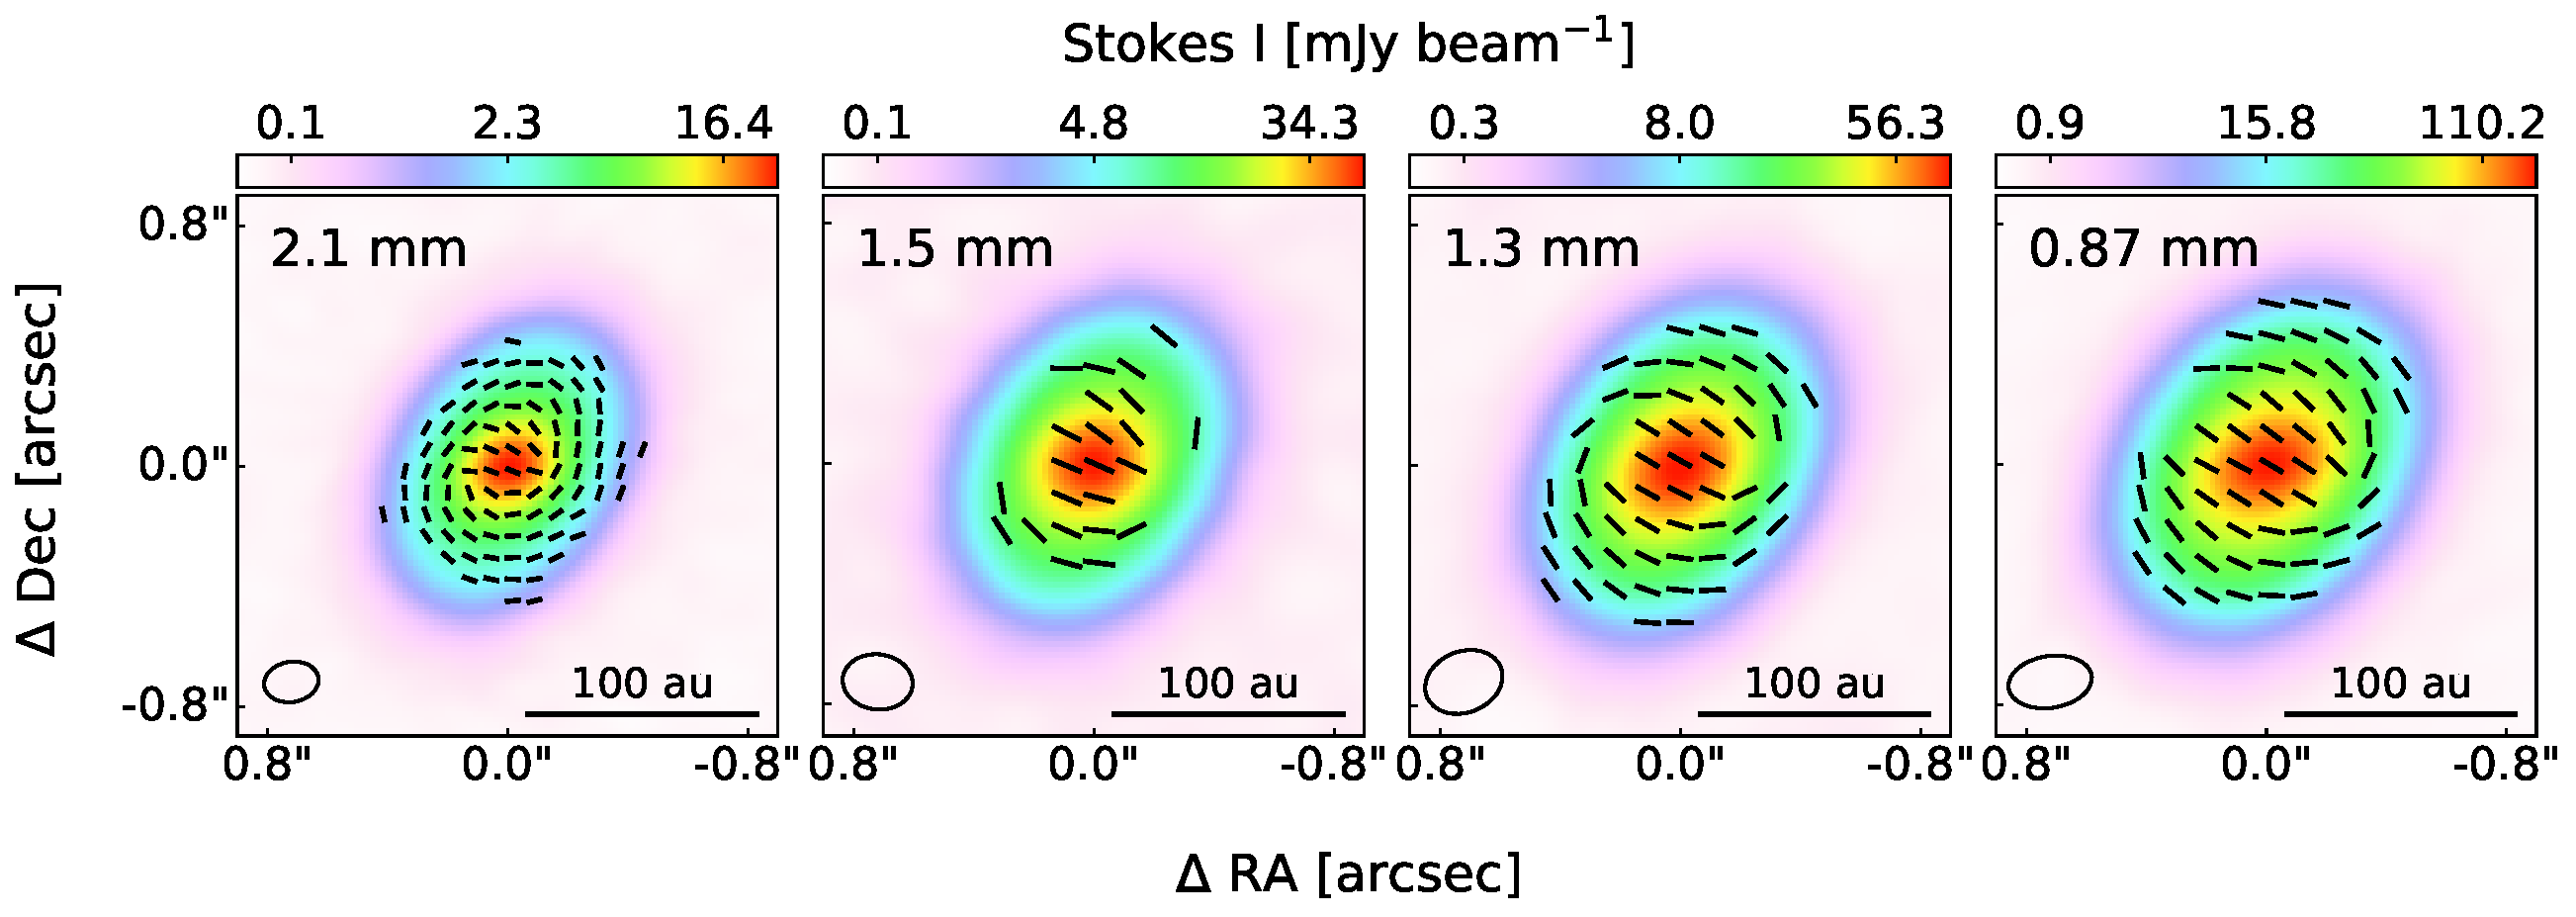
\includegraphics[width=\textwidth]{WRITEUP_AND_IMAGES/IMAGES/WRITEUP/StokesI_POLI/StokesI_grid_robust_minus1_Delta_stretched.pdf}

    \vspace{0.5cm}

    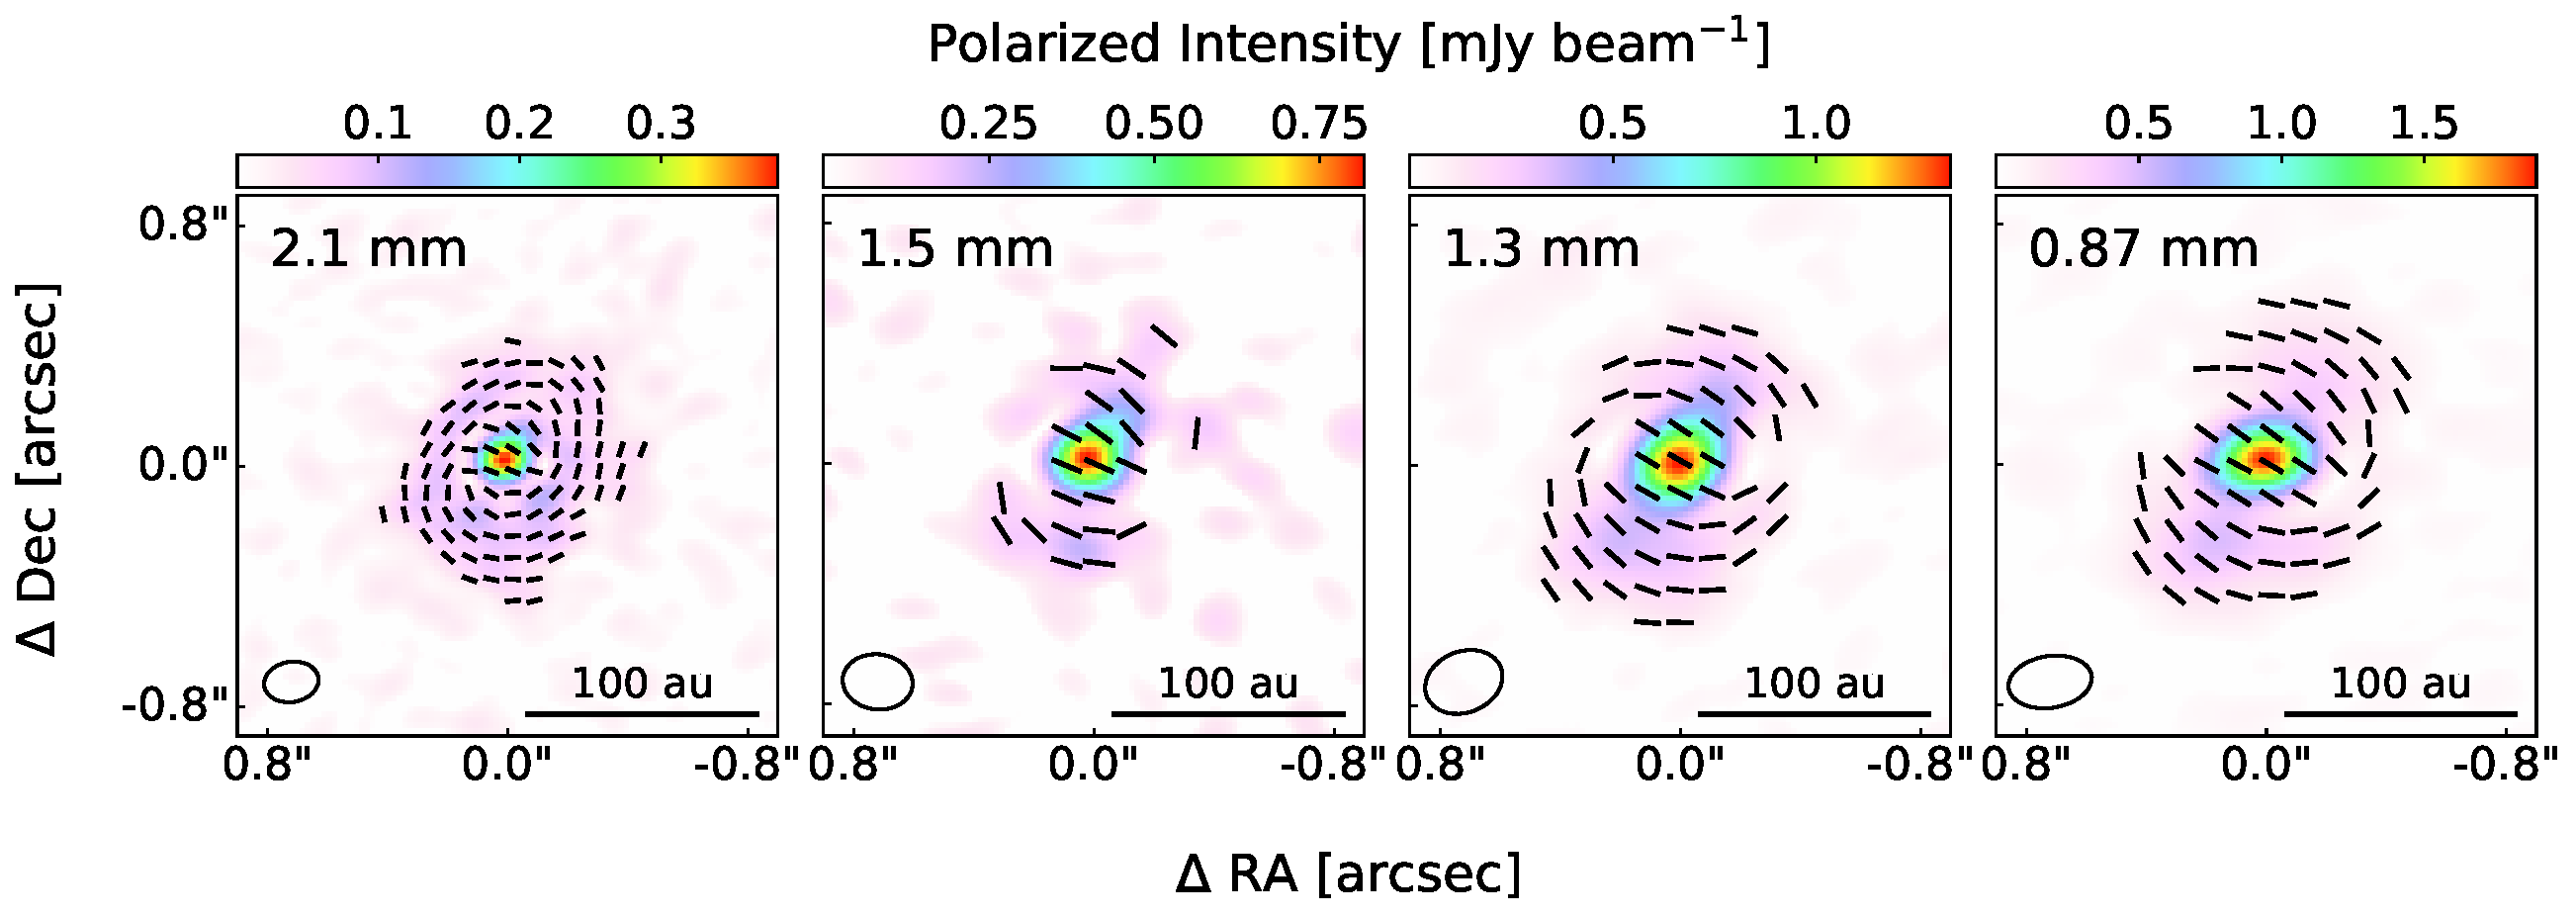
\includegraphics[width=\textwidth]{WRITEUP_AND_IMAGES/IMAGES/WRITEUP/StokesI_POLI/POLI_grid_robust_minus1_Delta.pdf}
    \caption[\SI and polarized intensity images with polarization vectors.]{Grid of images at each wavelength showing (top) \SI emission and (bottom) debiased polarized intensity. Polarization vectors are overlaid as black lines of equal length, showing the change in morphology with wavelength. Vectors are shown only for pixels that satisfy the criteria described in Chapter \ref{sec: methods_vector_criteria}. The beam is shown in the lower left corner, and a reference scale of 100 au is shown in the top right corner.  }% \later{scale vectors by POLF. make a separate 2 X 2 panel plot so that the polarization segment lengths are easier to see.} }
    \label{fig: StokesI_POLI_grid}
\end{figure}



% The streamer at \bfive is highlighted in red vectors, and is explained further in Chapter \ref{chap: discussion_streamer}
% ----------------------------



In Figure \ref{fig: StokesI_POLI_grid}, we present the cleaned \SI and debiased polarized intensity images of IRS 63 at \bfourNS, \bfiveNS, \bsixNS, and \bsevenNS, overlaid with the polarization vectors that show the observed polarization morphology. At each wavelength, all vectors are normalized to the same length to focus on the polarization angle rather than magnitude. 



As the observing wavelength decreases, there is a clear transition in polarization morphology. At \bfourNS, the polarization vectors are mostly azimuthal, following a circular pattern around the centre of the disk. This morphology is consistent with the pattern expected from aligned dust grains (e.g., via radiative alignment or aerodynamic alignment, see Chapter \ref{sec: intro_polarization_mechanisms}), as shown in Figure \ref{fig: kataoka_polarization_morphologies}(b). However, a small region at the centre of the disk shows that polarization vectors are aligned with the disk minor axis. As the wavelength decreases from \bfour to \bsevenNS, this minor axis-aligned region increases, while the azimuthal pattern gets pushed to the outer disk. The polarization morphologies at \bfive and \bsix are intermediate between the two patterns, but at \bseven the polarization vectors are mainly aligned with the disk minor axis. This uniform, minor-axis-aligned polarization morphology is consistent with dust self-scattering, as shown in Figure \ref{fig: kataoka_polarization_morphologies}(c). These observed morphologies motivate the geometric models considered in Chapter \ref{sec: methods/modelling polarization pattern}. 
% ------------------------------------------------------------------




% ------------------------------------------------------------------
\section{Intensity Profiles}
\label{sec: ch4_intensity_profiles}
% ------------------------------------------------------------------
To study the structure of IRS 63, intensity profiles were extracted along the minor axis in both \SI and debiased polarized intensity at each wavelength. Figure \ref{fig: slice-along-minor} shows the locations of the slices at each wavelength.




% ------------------------------------------------
\begin{figure}[htbp]
  \centering
  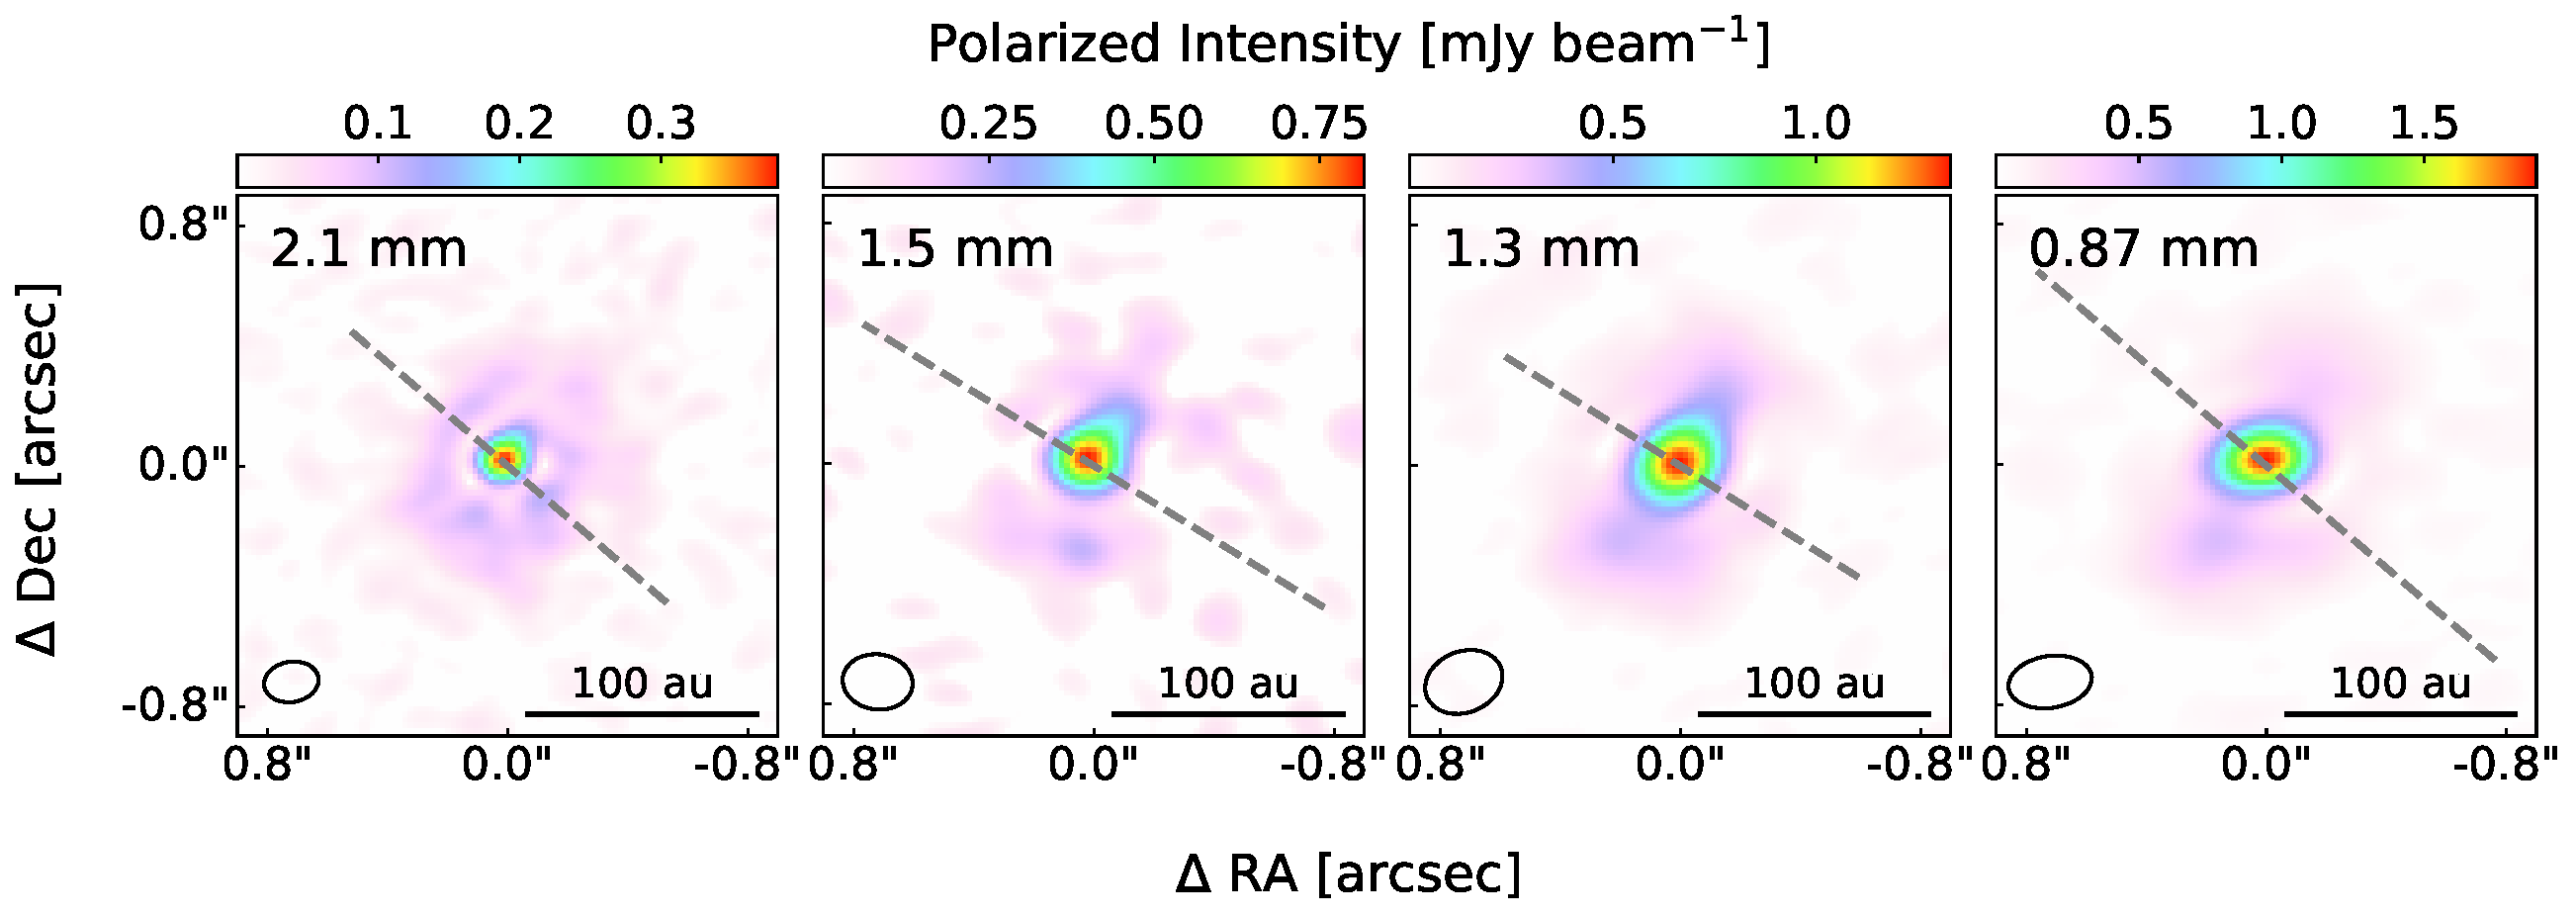
\includegraphics[width=0.99\textwidth]{WRITEUP_AND_IMAGES/IMAGES/WRITEUP/Slices/MinorAxisSliceGrid_robust_minus1_Delta.pdf}
  \caption[Locations of the minor-axis slices.]{Locations of the minor-axis slices extracted from the images at each wavelength. The same slice was used for both \SI and debiased polarized intensity.  }
  \label{fig: slice-along-minor}
\end{figure}
% ------------------------------------------------




The slices in \SI and polarized intensity for each wavelength are presented in Figure \ref{fig: slices_grid}. The synthesized beam for each wavelength is overplotted for comparison. The beam is plotted as a one-dimensional Gaussian, with a standard deviation calculated from the beam full width at half maximum (FWHM) along the minor axis using: 
\begin{equation}
    \sigma = \frac{\text{FWHM}}{2\sqrt{2 \ln{2}}}.
    \label{eq: FWHM_to_sigma}
\end{equation}
\noindent The Gaussian was normalized to 1 and scaled by the peak intensity of each slice. 
% \noindent The standard deviations are used to calculate the Gaussian shape at each offset using:
% \begin{equation}
%     \text{Beam(offset)} = \exp{\left(-\frac{\text{offset}^2}{2\sigma^2}\right)},
% \end{equation}
% \noindent which was then normalized to 1 and scaled by the maximum value of the slice. 




The \SI profiles (top row of Figure \ref{fig: slices_grid}) show a single peak at the centre of the disk at all four wavelengths. This is expected, as the density of the disk increases towards the central star, resulting in stronger emission from the inner disk. The angular resolution of these data is not sufficient to resolve the rings seen in \cite{Dom2020} (Figure \ref{fig: IRS63_Dom_Sadavoy}, left panel). However, in the debiased polarized intensity profiles (bottom row of Figure \ref{fig: slices_grid}), we do not see the same trend. The profiles are consistently offset from the centre position at all four wavelengths. Relative to the synthesized beam, the offset is not well resolved.  Nevertheless, having the offset is consistent across all four wavelengths indicates it is a real feature.





An offset in polarized intensity relative to total intensity could be a geometric effect due to the disk being both puffy and inclined. \cite{Yang} showed that optically thick disks that are both flared and inclined should have brighter polarized intensities on the near side of the disk.  This difference is due to forward scattering (from the near side) being favoured over back scattering (from the far side).  Thus, Figure \ref{fig: slices_grid} demonstrates that IRS 63 is likely flared, meaning its vertical scale height increases with radius (Figure \ref{fig: dust-grain-growth-schematic}). Unfortunately, the angular resolution of the data is insufficient to further model the polarization intensity and constrain the flaring.









\begin{figure}[htbp]
  \centering
  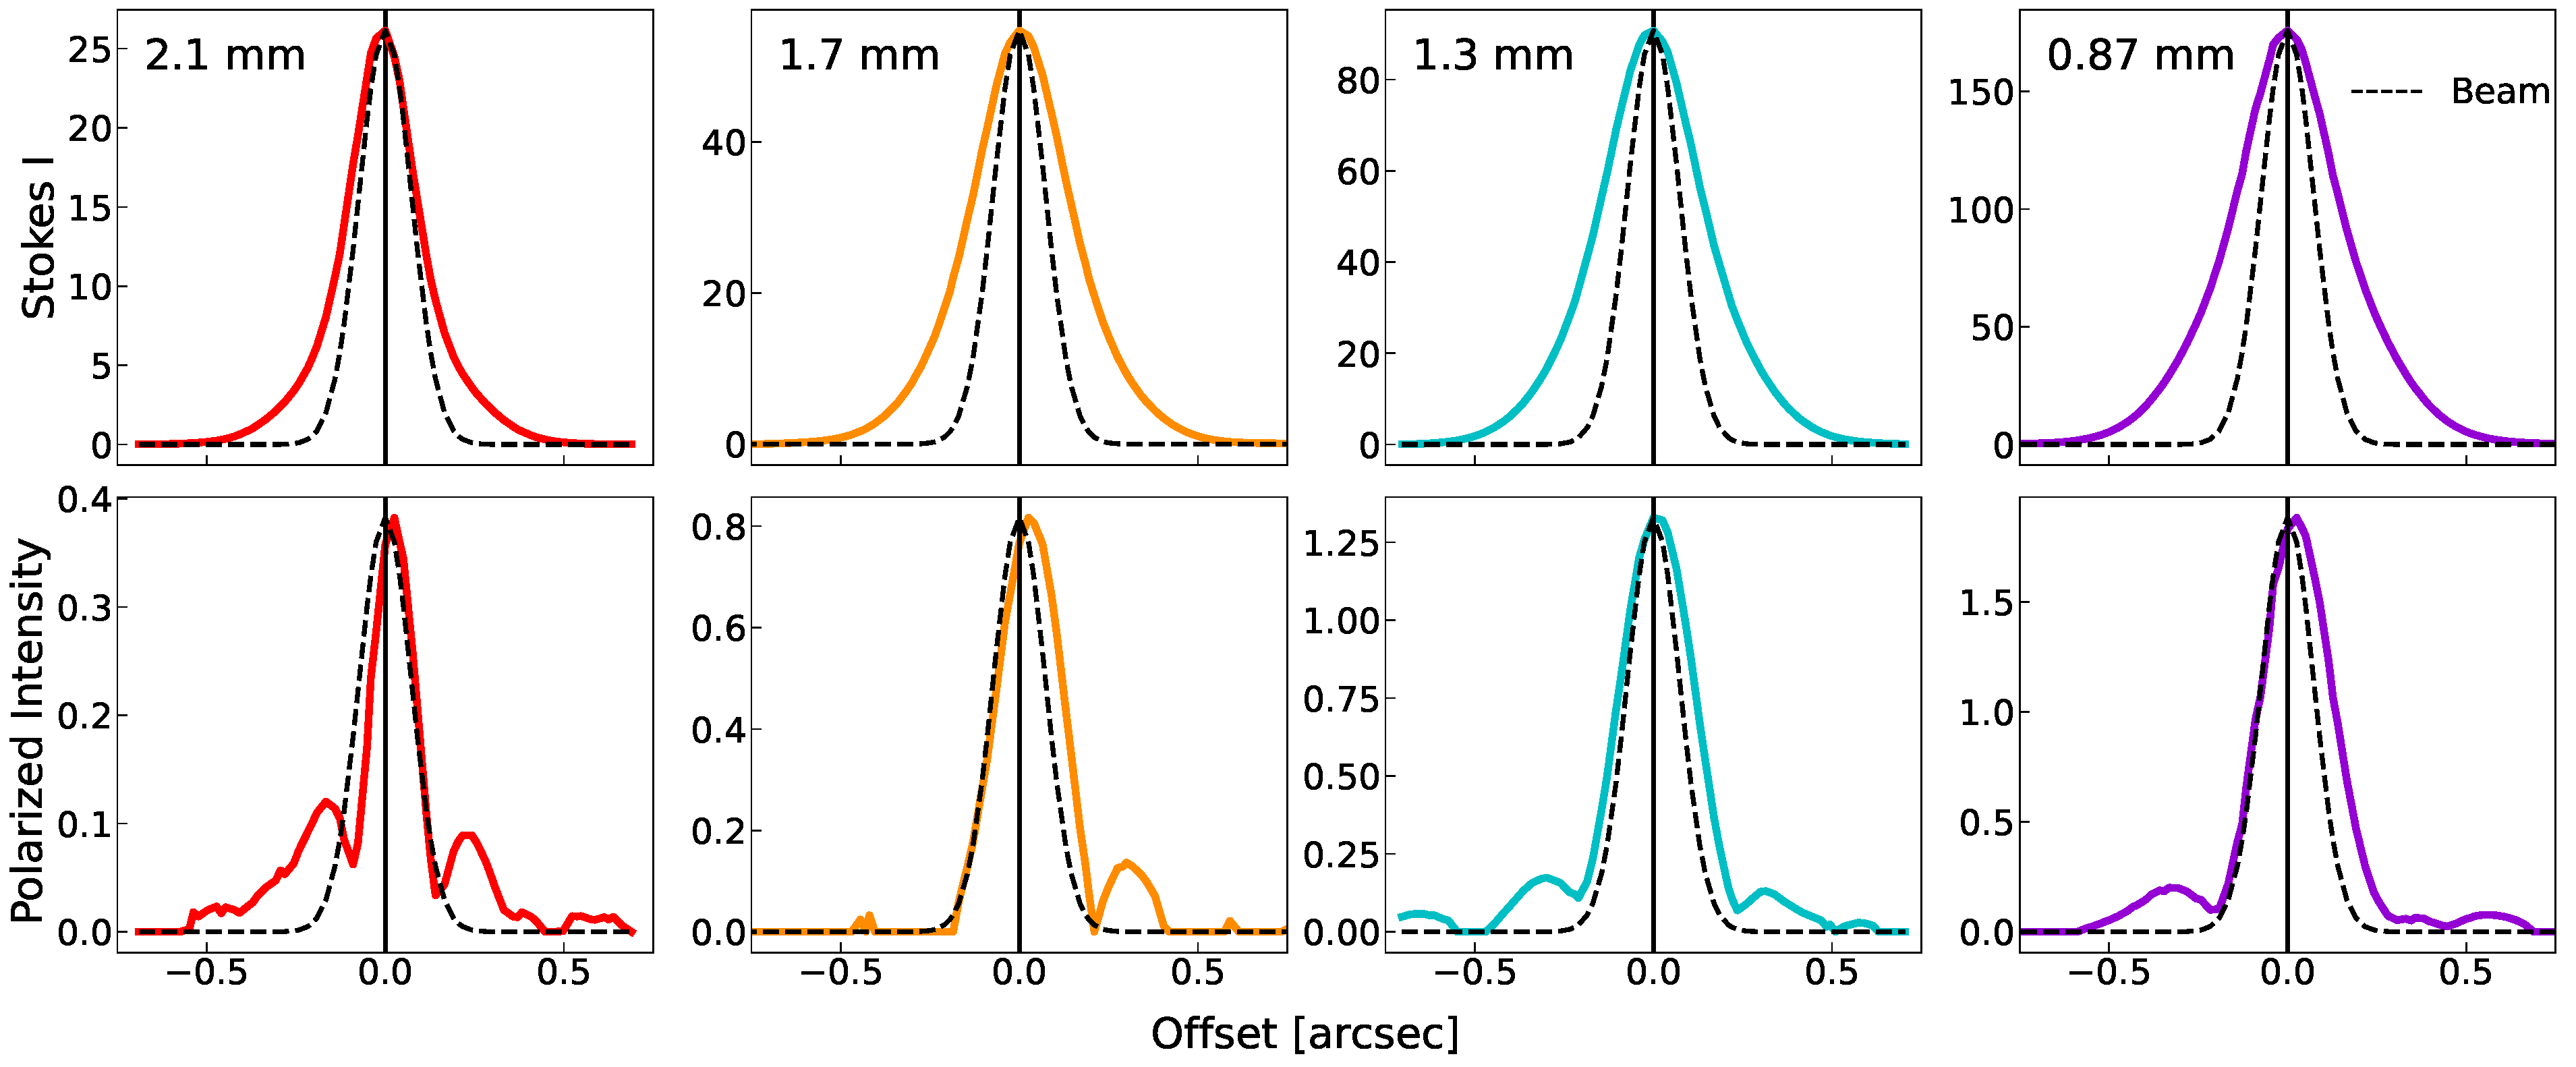
\includegraphics[width=0.99\textwidth]{WRITEUP_AND_IMAGES/IMAGES/WRITEUP/Slices/MW_slices_GRID.pdf}
  \caption[\SI and debiased polarized intensity profiles.]{Plot of (top) \SI and (bottom) debiased polarized intensity offset as a function of the offset from the centre position of the disk, both in units of mJy beam$^{-1}$. The centre position is shown as a solid black line, with the corresponding values found in Table \ref{tab: source_info}. The slices used for these profiles are shown in Figure \ref{fig: slice-along-minor}. }
  \label{fig: slices_grid}
\end{figure}




% ------------------------------------------------------------------

% ------------------------------------------------------------------
\section{Geometric Modelling of Polarization Pattern}
\label{sec: methods/modelling polarization pattern}
% ------------------------------------------------------------------


To quantify the observed polarization morphologies, they were modelled using two geometric models. This approach is motivated by the work done of \cite{Stephens_2017}, who used a similar approach to model the polarization morphology of HL Tau. The models were created to reproduce the observed polarization structure, including azimuthal patterns (Figure \ref{fig: kataoka_polarization_morphologies}a), polarization vectors that uniformly align with the minor axis (Figure \ref{fig: kataoka_polarization_morphologies}b), and intermediate morphologies. \SQ and $U$ maps were made for the two extreme polarization cases (purely azimuthal and purely uniform) at each pixel, as shown in Figure \ref{fig: StokesI_POLI_grid}, and combined to produce the intermediate cases. Since dust self-scattering is expected to produce a uniform pattern, the model allows us to identify the regions of the disk where scattering-induced polarization may dominate. 

A more physical model could include radiative transfer. The goal here is to identify the regions of the disk where the signatures of each polarization mechanism dominate, rather than to model the physical mechanisms that produce the observed patterns. The two geometric models are described in Chapters \ref{sec: ch4_ratio_model} and \ref{sec: ch4_gaussian_model}.


% ----------------------------------------------------------
\subsection{Goodness of Fit}
% ----------------------------------------------------------

To determine how well a geometric model reproduced the polarization observations, a chi-squared value was calculated. First, the difference between the observed and model-predicted polarization angle needed to be calculated carefully. Polarization angles can range from 0--180\degg because polarization measures orientation, rather than direction. The polarization vectors have a 180\degg ambiguity such that a vector with a polarization angle of 0\degg looks the exact same at a polarization angle of 180\deggNS. As a result, two polarization angles that are physically very similar can have a large numerical difference. For example, polarization angles of 1\degg and 179\degg only differ by 2\deggNS, but directly taking their difference would give 178\deggNS. To account for this ambiguity, the angular difference is defined by the minimum angular separation between the two angles:
\begin{equation}
    \Delta \theta = \text{min}(|\theta_{\text{obs}} - \theta_{\text{model}}|, 180\deggEQ - |\theta_{\text{obs}} - \theta_{\text{model}}|),
    \label{eq: minimum_separation}
\end{equation}

\noindent where $\theta_{\text{obs}}$ is the observed polarization angle and $\theta_{\text{model}}$ is the polarization angle predicted by either the ratio or Gaussian model. The angular differences were then used to calculate the chi-squared value:
\begin{equation}
    \chi^2 = \sum \left(\frac{\Delta \theta_i}{\sigma_\theta}\right)^2,
    \label{eq: chi_sq}
\end{equation}
\noindent where the angular distance is summed over all sampled polarization vectors, and \PAerr is the uncertainty in the observed polarization angle.  

The value of $\chi^2$ was then converted to reduced chi-squared by:
\begin{equation}
    \chi^2_{reduced} = \frac{1}{n-k} \times \chi^2,
    \label{eq: chi_sq_reduced}
\end{equation}
\noindent where $n$ is the number of sampled polarization vectors and $k$ is the degrees of freedom. For the ratio model (Chapter \ref{sec: ch4_ratio_model}), there is one degree of freedom, and for the Gaussian method (Chapter \ref{sec: ch4_gaussian_model}), there are three ($\phi$, $b$, and $a$). 
% ----------------------------------------------------------

% ----------------------------------------------------------
\subsection{Ratio Model}
\label{sec: ch4_ratio_model}
% ----------------------------------------------------------
The first geometric model tested is the \emph{ratio model}, which is more similar to the approach used in \cite{Stephens_2017}. The main idea behind this model is to reproduce the observed polarization morphologies, ranging from purely aligned with the minor axis of the disk to purely azimuthal, along with intermediate cases. This was achieved by creating a grid of models weighted between these two extreme cases. 


The first extreme case, 100\% uniform pattern, we modelled the disk where every vector is aligned with the minor axis of the disk (90\degg from the disk position angle, Table \ref{tab: source_info}). For the second extreme case, 100\% azimuthal pattern, we modelled the polarization vectors to follow a circular pattern around the centre of the disk. The centre point of the disk at each wavelength can be found in Table \ref{tab: source_info}. For each pixel $(x, y)$, we calculated the azimuthal polarization angle relative to the disk centre using \texttt{numpy.arctan2}.


Figure \ref{fig: RatioExamples} shows examples of the models created using the ratio method.  The left-most and right-most panels show the two extreme cases of 100\% uniform polarization and 100\% azimuthal polarization, respectively.  The middle panel shows an intermediate case that is 50\% uniform and 50\% azimuthal.  To create the intermediate cases, models were generated in steps of 10\% and are denoted as $N \uni + (100 - N) \azi$, where $N = 0, 10 \ldots, 100$. Here, Uni and Azi represent the pure uniform and pure azimuthal cases, respectively, and $N$ gives the percentage contribution of the uniform case. 


% the offset from the disk centre $(x_c, y_c)$ is calculated as:
% \begin{equation}
% \begin{aligned}
%     \delta x &= x - x_c, \\
%     \delta y &= y - y_c.
% \end{aligned}
% % \label{eq: vectors}
% \end{equation}



Since polarization angles cannot be directly added to find the intermediate cases, we instead generated mock \SQ and $U$ maps and combined those in the appropriate fractions.  We first solved for the \SQ and \SQ maps for the extreme cases. (100Uni + 0Azi and 0Uni and 100Azi) using:
\begin{equation}
\begin{aligned}
Q_{\text{Uni}} &= \rho I \cos(2\theta_{\text{Uni}}) \text{ and }
Q_\text{Azi} = \rho I \cos(2\theta_\text{Azi}),
     \\
U_{\text{Uni}} &=  \rho I \sin(2\theta_{\text{Uni}}) \text{ and }
U_\text{Azi} =  \rho I \sin(2\theta_\text{Azi}) 
\end{aligned}
% \label{eq:50U50A}
\end{equation}
\noindent following \cite{Montier}, where $\rho$ is the average polarization fraction over the centre and edges, which we fixed at 2\%. This value is representative of an intermediate case between the two morphologies, likely overestimating the polarization fraction for the uniform pattern and underestimating it for the azimuthal pattern. 


%This is consistent with values of 0.02-0.03 from \cite{Kataoka_2017}, 



The intermediate \SQ and $U$ maps were then obtained by combining the two extreme models using:
\begin{equation}
\begin{aligned}
Q_{N}
    &= \frac{N}{100}\,Q_{\text{Uni}}
     + \frac{100 -N}{100}\,Q_{\text{Uni}}, \\
U_{N}
    &= \frac{N}{100}\,U_{\text{Uni}}
     + \frac{100 -N}{100}\,U_{\text{Azi}}.
\end{aligned}
% \label{eq:50U50A}
\end{equation}

\noindent The resulting $Q_N$ and $U_N$ model maps were used to calculate the model polarization angle at each pixel using Equation \ref{eq: PA}. The polarization vectors were generated using the methods in Chapter \ref{sec: chap4_polarization_vectors}. This process was repeated for each ratio combination. For example, $N=50$ corresponds to the $50\uni+50\azi$ model, shown in the middle panel of Figure \ref{fig: RatioExamples}.





\begin{figure}[htbp]
  \centering
  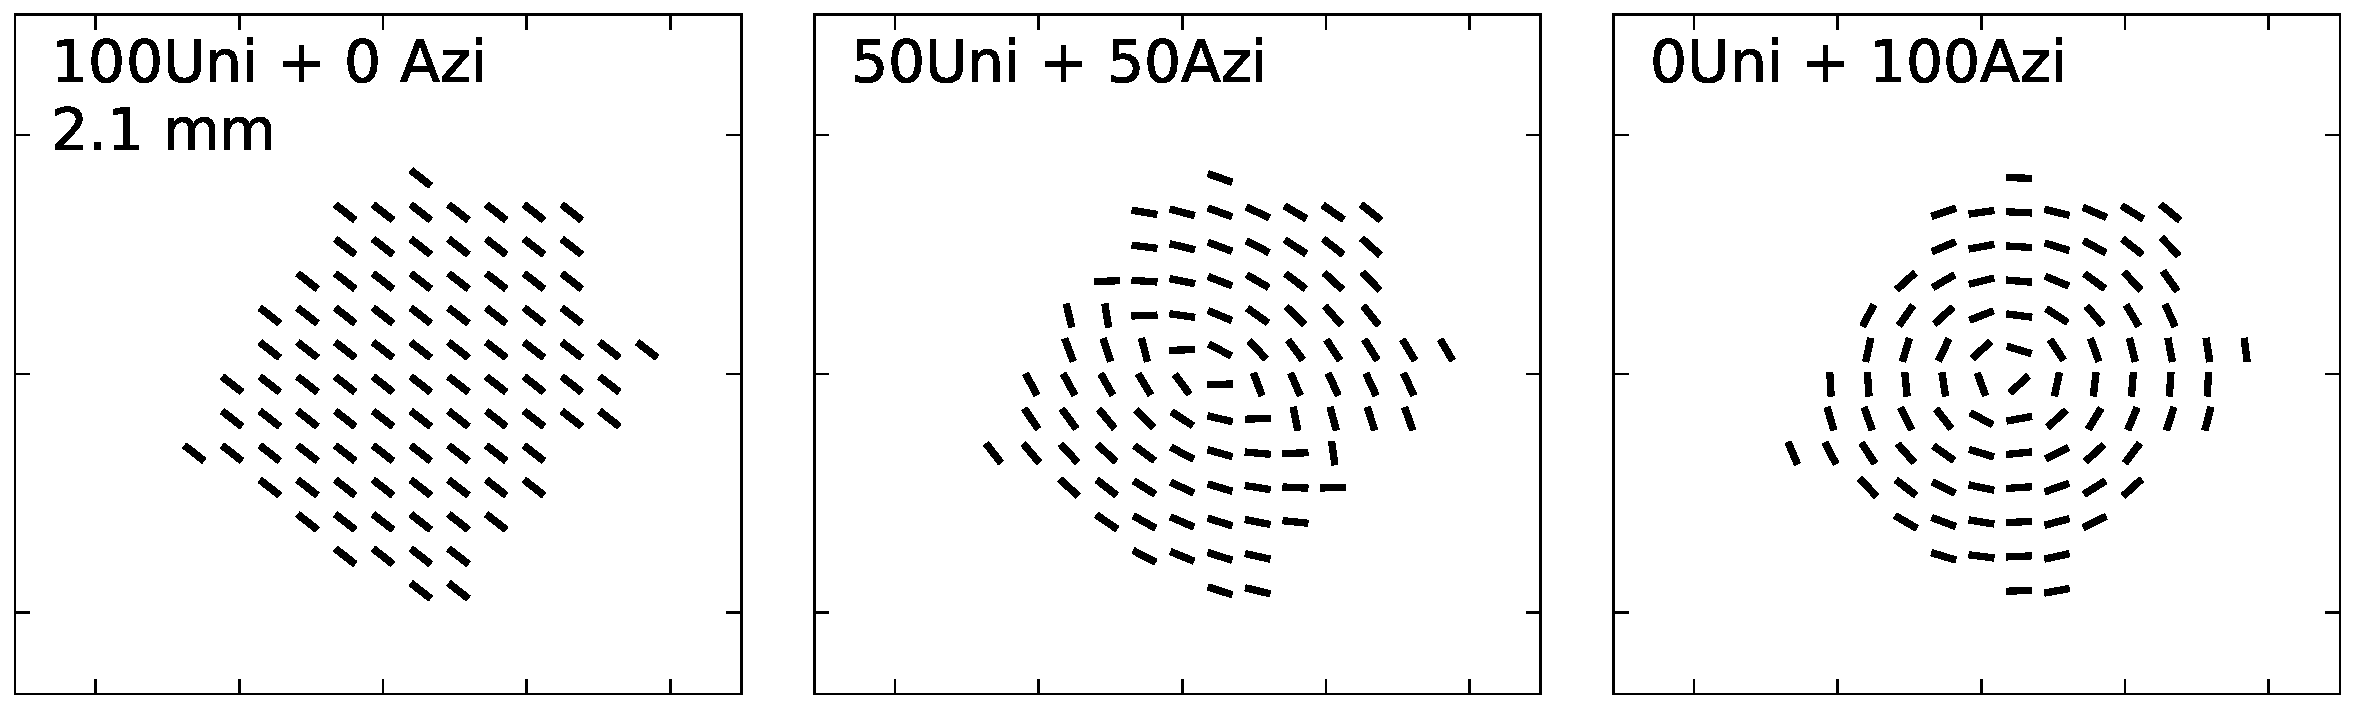
\includegraphics[width=0.99\textwidth]{WRITEUP_AND_IMAGES/IMAGES/WRITEUP/Ratio/RatioExamplesTest_Band4_NoAxes.pdf}
  \caption[Example of the $N = 100, N=50$ and $N = 0$ cases of the ratio model.]{Example of the $N = 100, N=50$ and $N = 0$ cases of the ratio model for \bfourNS.}
  \label{fig: RatioExamples}
\end{figure}





For the ratio models, Table \ref{tab:ratio_model_chi2} presents the \chired values calculated for each test with the best-fit value shown in bold.  Figure \ref{fig: RatioBestGrid} shows the best-fit model with the observed vectors in black and the model vectors in red.


Taking \bfive as an outlier (see Chapter \ref{sec: discussion_band5_data_issues}), the best-fit ratio models show that, as wavelength decreases, the observations are better matched with a higher uniform contribution. This result is consistent with the observations discussed in Chapter \ref{sec: c4_polarization_maps}, which show a greater uniform contribution with decreasing wavelength. 






% This was updated to Band 5 robust = -1 on July 18th
% These numbers might need to be changed if we change how we calculate chi^2
% This is Band 4 nterms2, Band 7 nterms 2.
\begin{table}[h!]
\centering
\caption[Ratio model fitting results.]{Ratio model fitting results for each wavelength. }
\begin{tabular}{lcccc}
\toprule
\textbf{Ratio Model} & \textbf{\bfour} & \textbf{\bfive} & \textbf{\bsix} & \textbf{\bseven} \\
\midrule
100Uni + 0Azi
& 181.67 % Band 4 
& \textbf{22.58} % Band 5 
& 37.39 % Band 6  
& \textbf{79.12} \\


90Uni + 10Azi
& 171.40 % Band 4
& 24.22 % Band 5  
& 33.93 % Band 6  
& 88.59 \\

80Uni + 20Azi
& 158.01 % Band 4 
& 27.77 % Band 5  
& \textbf{33.36} % Band 6  
& 108.65 \\

70Uni + 30Azi
& 140.74 % Band 4 
& 34.28 % Band 5  
& 37.99 % Band 6 
& 144.84 \\

60Uni + 40Azi
& 116.11 % Band 4 
& 45.10 % Band 5
& 51.96 % Band 6 
& 206.76 \\

50Uni + 50 Azi
& \textbf{88.21} % Band 4 
& 63.81 % Band 5  
& 84.48 % Band 6  
& 322.01 \\

40Uni + 60Azi
& 124.99 % Band 4 
& 91.17 % Band 5  
& 140.41 % Band 6  
& 498.43 \\

30Uni + 70 Azi
& 131.03 % Band 4 
& 116.35 % Band 5
& 191.20 
& 647.50 \\

20Uni + 80Azi
& 133.70 % Band 4 
& 138.36 % Band 5  
& 233.90 % Band 6  
& 776.00 \\

10Uni + 90Azi
& 136.42 % Band 4
& 157.27 % Band 5  
& 270.41 % Band 6 
& 886.40 \\

0Uni + 100Azi
& 139.41
& 173.26
& 302.34 
& 979.97 \\
\bottomrule
\end{tabular}
\begin{tablenotes}
% \footnotesize
\item \textbf{Note:} Goodness-of-fit quantified by $\chi^2_{reduced}$ (Equation \ref{eq: chi_sq_reduced}). Best fits are shown in bold. 
\end{tablenotes}
\label{tab:ratio_model_chi2}
\end{table}






\begin{figure}[htbp]
  \centering
  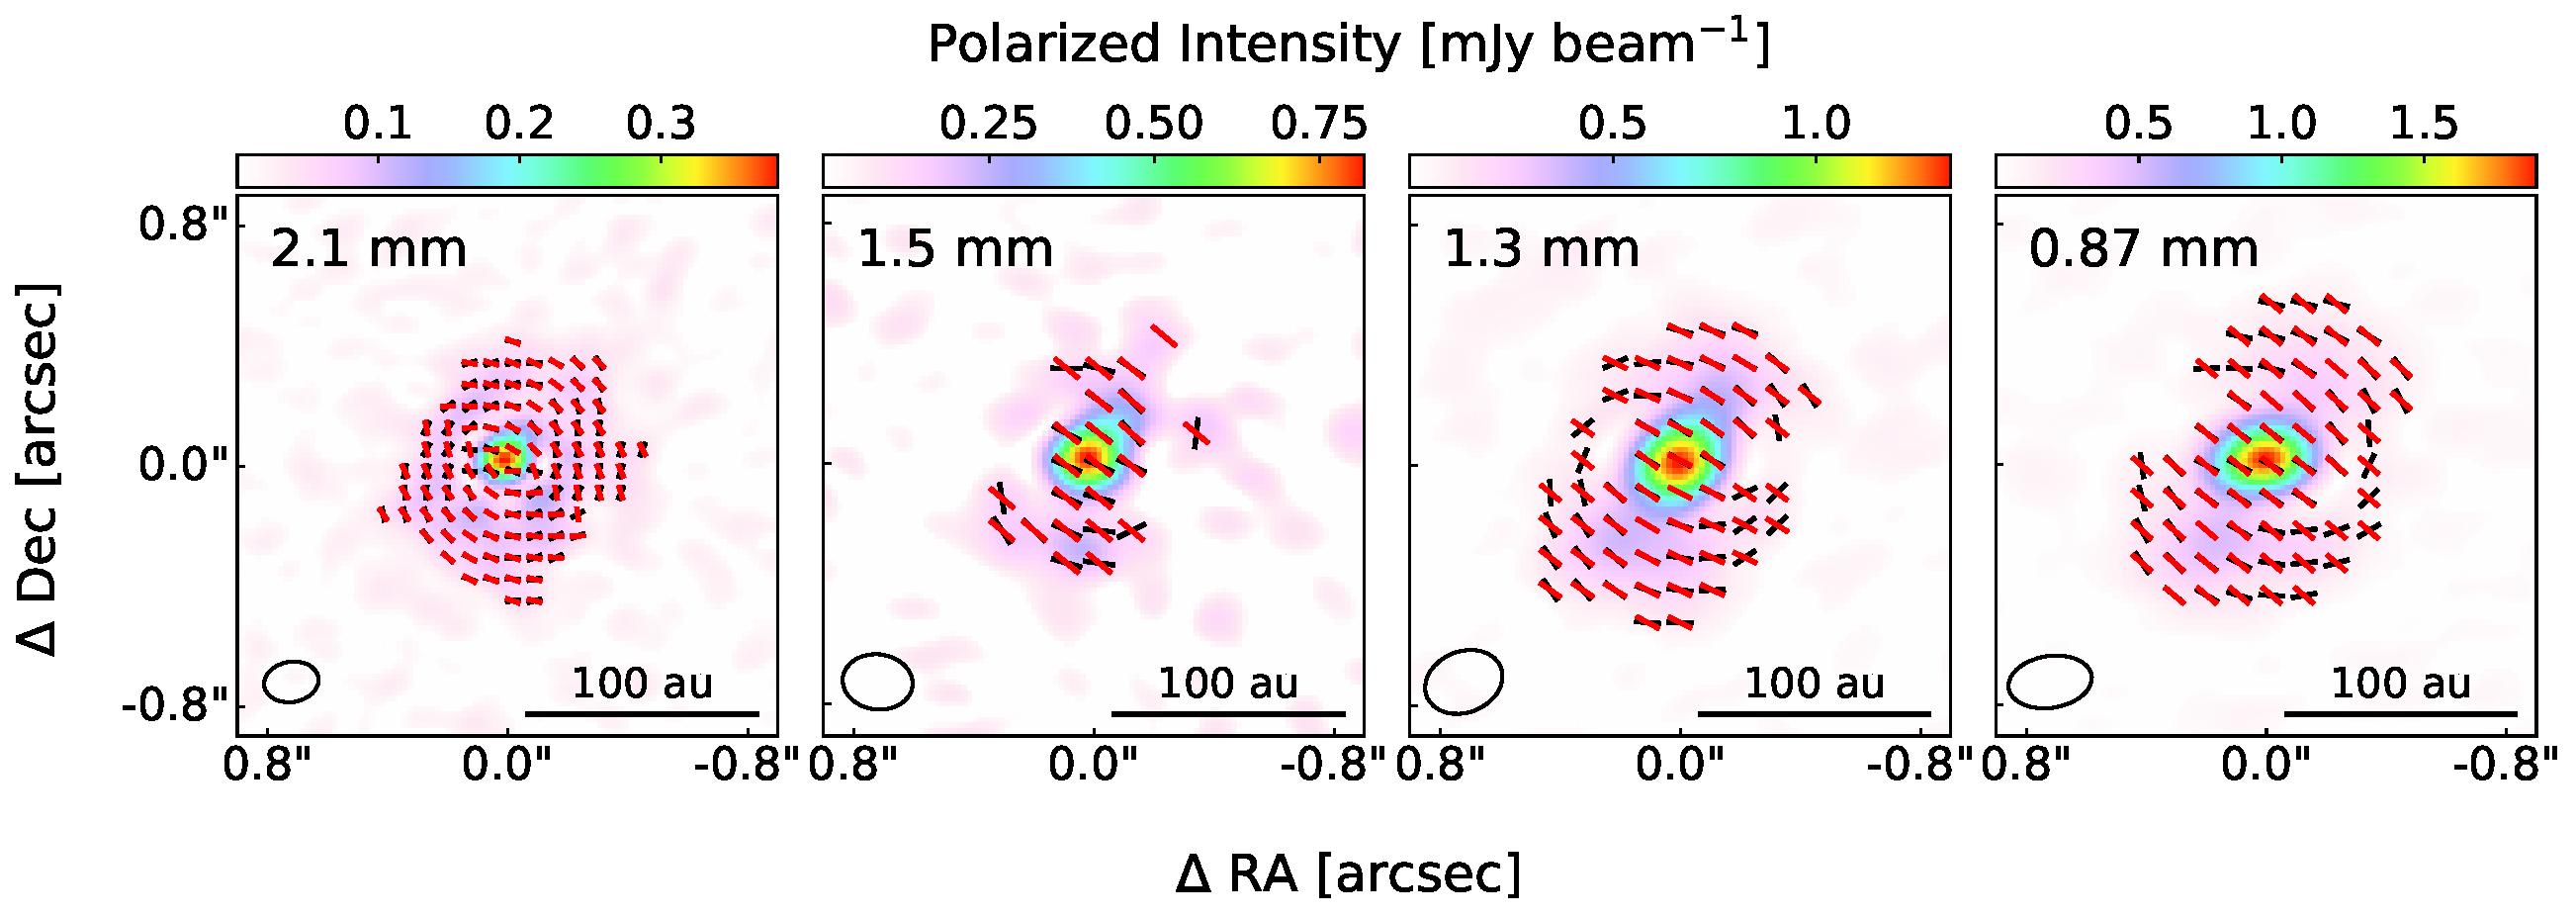
\includegraphics[width=0.99\textwidth]{WRITEUP_AND_IMAGES/IMAGES/WRITEUP/Ratio/Best_grid_Delta.pdf}
  \caption[Figure \ref{fig: StokesI_POLI_grid}, with the polarization vectors from the best-fit ratio model.]{Figure \ref{fig: StokesI_POLI_grid}, overplotted with the polarization vectors in red from the best-fit ratio model at each wavelength. The corresponding best-fit ratio models are listed in Table \ref{tab:ratio_model_chi2}.  }
  \label{fig: RatioBestGrid}
\end{figure}
% ----------------------------------------------------------






% ----------------------------------------------------------
\subsection{Gaussian Model}
\label{sec: ch4_gaussian_model}
% ----------------------------------------------------------


The second geometric model tested is the \emph{Gaussian model}. The aim of this model was to reproduce a polarization morphology that transitions from being aligned with the minor axis of the disk at the centre to becoming more azimuthal towards the outer parts of the disk. This is based on the expectation that the emission from the inner region is optically thick and would therefore be dominated by self-scattering \citep{Kataoka_2015}, with optical thickness decreasing towards the outer edge of the disk. 


To achieve this, we used a rotated 2-dimensional flat-topped Gaussian model with three free parameters: $\phi$, $a$ and $b$. The Gaussian was calculated using the equation:
\begin{equation}
W_{\text{Uniform}} =  I_0 
\exp\left[-\half \left(\left|\frac{X_{M}}{\sigma_M}\right|^\phi + \left|\frac{Y_{m}}{ \sigma_m}\right|^\phi\right)\right],
    \label{eq: gaussian_eq}
\end{equation}
\noindent where $I_0$, the peak value, was calculated using the equation:
\begin{equation}
    I_0 = \frac{1} {\sigma_m \sigma_M \sqrt{2\pi}}.
    \label{eq: Gaussian_model_I0}
\end{equation}

\noindent In Equation \ref{eq: gaussian_eq}, $\phi=2$ corresponds to a standard 2D Gaussian, while $\phi>2$ produces a flat-topped Gaussian. Table \ref{tab: gaussian_model_info} lists the parameters and the ranges we tested. The tested values of $a$ and $b$ control the widths of the Gaussian model (major and minor axes of the Gaussian, respectively), with each treated as the FWHM and converted to standard deviations using Equation \ref{eq: FWHM_to_sigma}. Additionally, a condition of $b$ $\leqq $ $a$ was required to ensure the minor axis was smaller than the major axis. 


% \begin{equation}
% f(x) = A \exp{\left(-\left(\frac{(x-x_0)^2}{2\signa_X^2}\right)^P\right)}
%     \label{eq: super-Gaussian}
% \end{equation}
% \question{do I need to cite this? I got it from Wikipedia.}


\begin{table}[h!]
\centering
\caption{Summary of parameters and tested values in the Gaussian model.  }
\begin{tabular}{lll}
\toprule
\textbf{Property} &
\textbf{Meaning} &
\textbf{Tested Values}  \\
\midrule

$\phi$
& super-Gaussian exponent
& 2, 3, 4, 5, 6, 7\\


$a$ (pixels)
& major axis of Gaussian
& 10, 20, 30, 40, 50\\

$b$ (pixels)
& minor axis of Gaussian
& 10, 20, 30, 40, 50\\

\bottomrule
\end{tabular}
\label{tab: gaussian_model_info}
\end{table}


The Gaussian was rotated to align with the major axis of the disk, using the position angle of the disk (\PAns) given in Table \ref{tab: source_info}. The coordinates ($x, y$) were shifted with respect to the centre of the disk ($x_c, y_c$) and then rotated:
\begin{equation}
\begin{pmatrix}
X_M \\
Y_m
\end{pmatrix}
=
\begin{pmatrix}
\cos(\PAeq) & -\sin(\PAeq) \\
\sin(\PAeq) & \cos(\PAeq)
\end{pmatrix}
\begin{pmatrix}
x - x_c \\
y - y_c
\end{pmatrix}.
\label{eq:rotated_coordinates}
\end{equation}





\noindent The Gaussian was normalized to a maximum of 1 so that it could be used as a pixel weight. Equation \ref{eq: gaussian_eq} creates a map that specifies the weights for the Uniform polarization region of the disk, where the weight is 1 at the centre and drops to zero with radius.  We use 1 - \Wuni to give the weight for the azimuthal polarization morphology. These two maps act as our weights, rather than a constant like in the ratio model. 


The weighted \SQ and $U$ were calculated by:
\begin{equation}
\begin{aligned}
Q_{\text{Gaussian}}
    &= \WuniEQ \,Q_{\text{Uni}}
     + (1 - \WuniEQ)\,Q_{\text{Azi}}, \\
U_{\text{Gaussian}}
    &= \WuniEQ\,U_{\text{Uni}}
     + (1 - \WuniEQ)\,U_{\text{Azi}},
\end{aligned}
% \label{eq:50U50A}
\end{equation}

\noindent As in the ratio model, the maps of $Q_{\text{Gaussian}}$ and $U_{\text{Gaussian}}$ were used to calculate the position angle (Equation \ref{eq: PA}). Figure \ref{fig: Methods/GaussianExamples} shows two example Gaussian weight maps with polarization vectors overlaid.  The values of $\phi$, $a$, and $b$ are given in the lower-left corner.  The vector sampling is selected to match the \bfour data.


\begin{figure}[htbp]
  \centering
  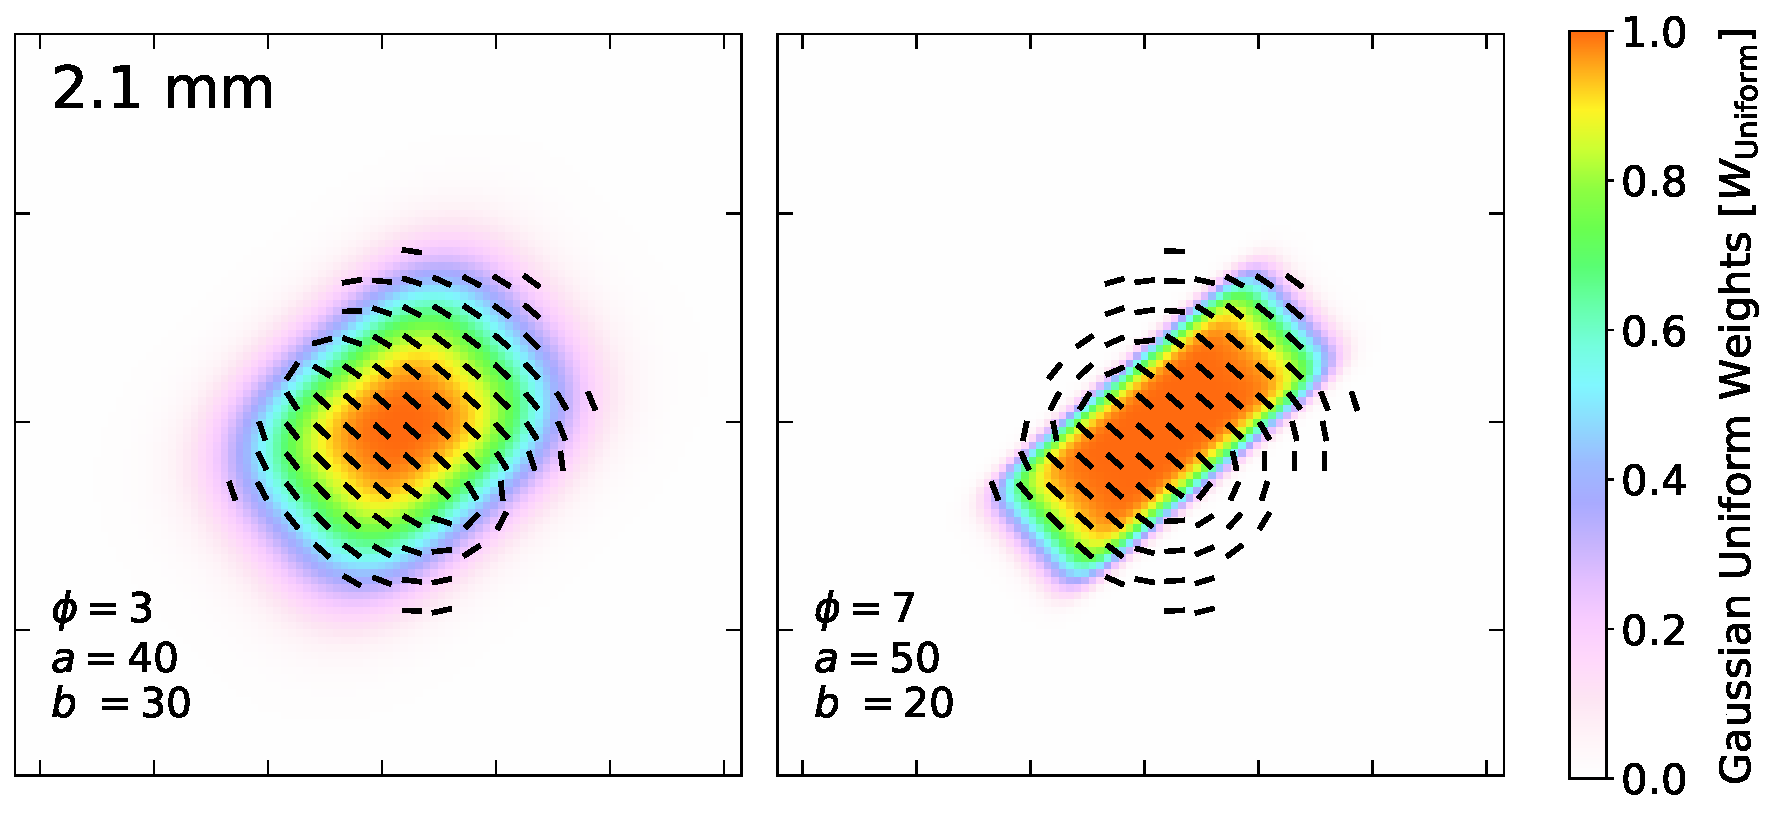
\includegraphics[width=0.8\textwidth]{WRITEUP_AND_IMAGES/IMAGES/WRITEUP/Gaussian/CustomExamples_B4.pdf}
  \caption[Two examples of the Gaussian weights for selected values.]{Two examples of the Gaussian weights for selected values of $\phi$, $a$ and $b$. }
  \label{fig: Methods/GaussianExamples}
\end{figure}





% ----------------------------------------------------------




For the Gaussian model, Table \ref{tab:gaussian_top5} presents the five best-fitting cases (out of 150 tested per wavelength) with the best-fit model highlighted in bold.  Figure \ref{fig: GaussianBestGrid} compares the observed and model vectors for the best-fit models at each wavelength. 




\begin{figure}[htbp]
  \centering
  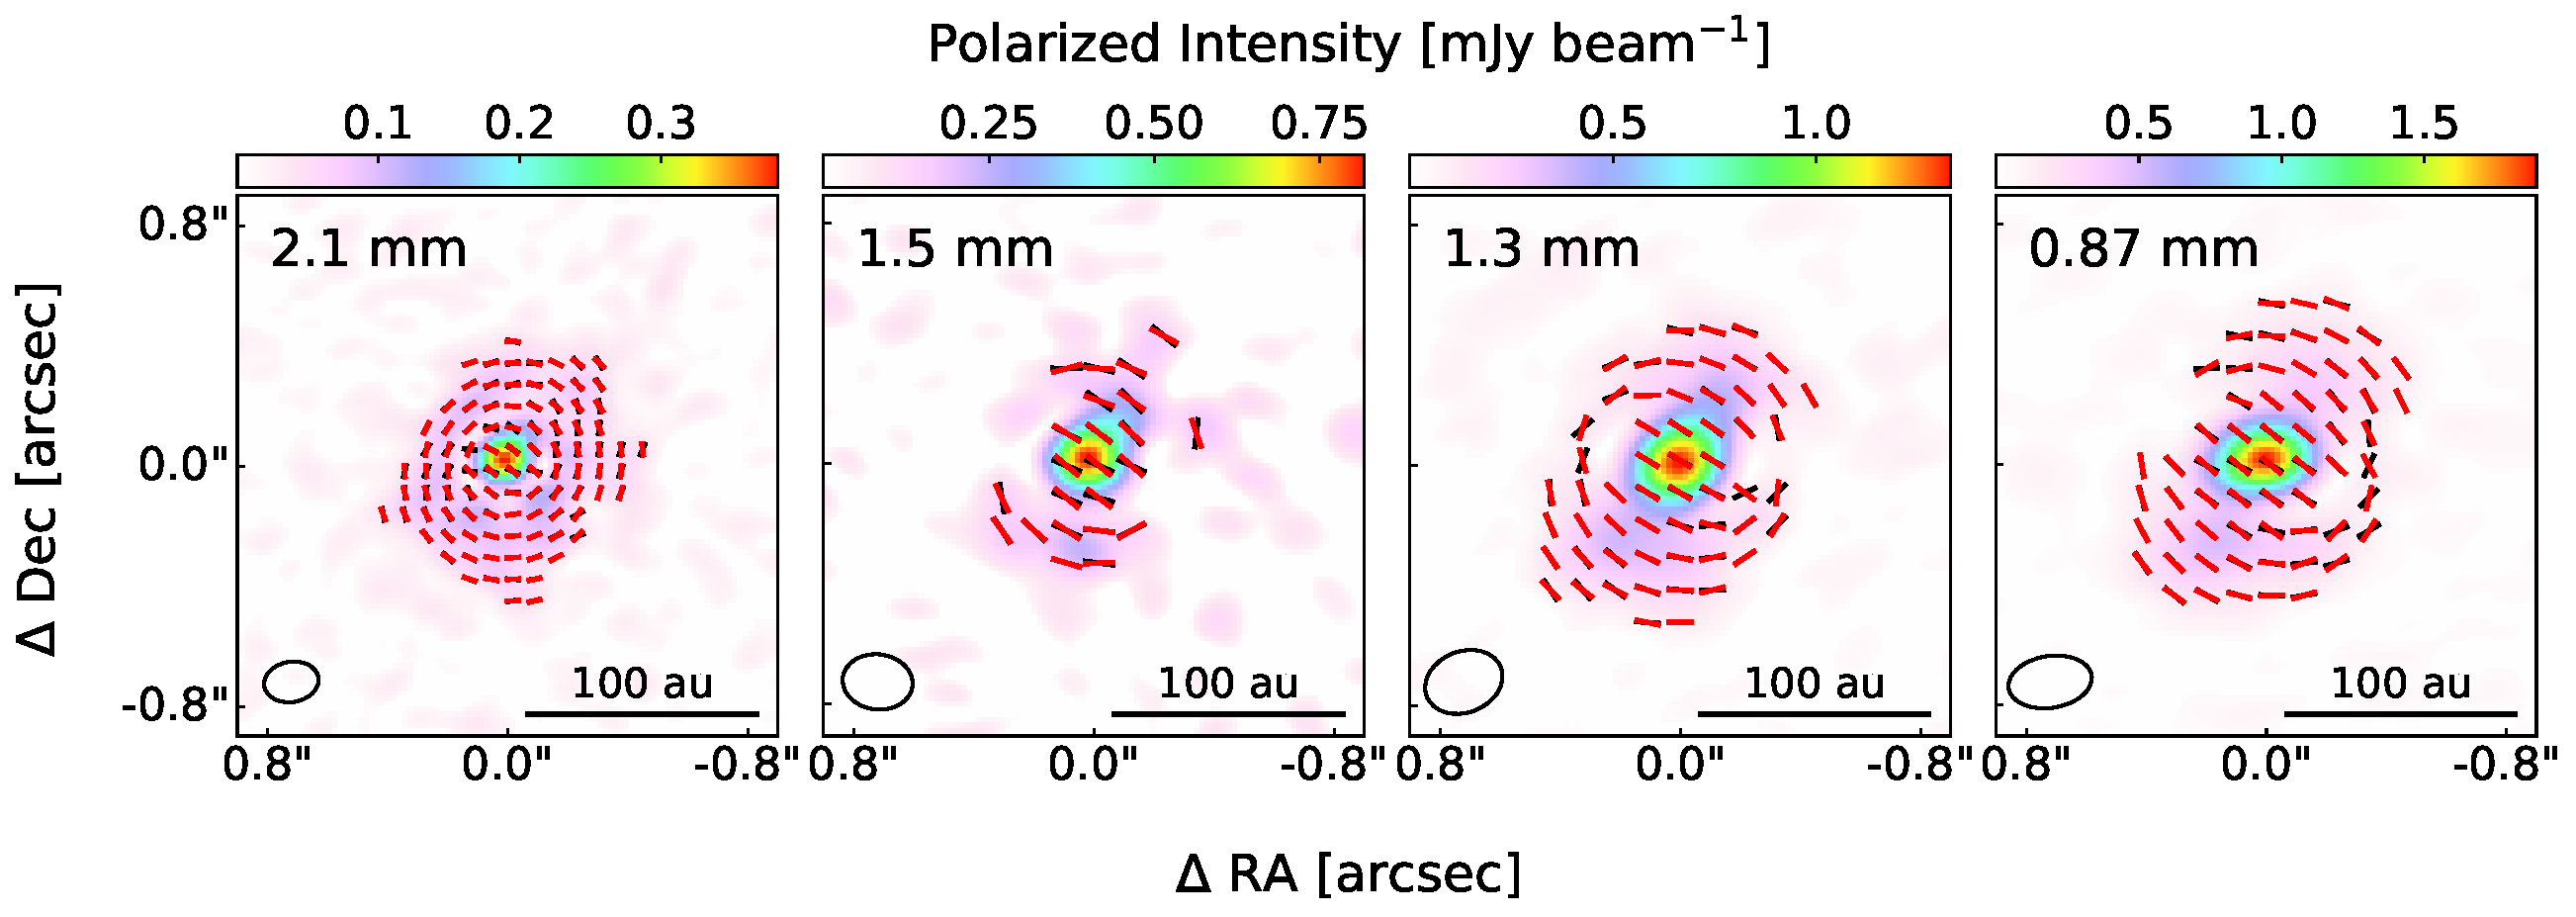
\includegraphics[width=0.99\textwidth]{WRITEUP_AND_IMAGES/IMAGES/WRITEUP/Gaussian/Best_grid_Delta.pdf}
  \caption[Same as Figure \ref{fig: RatioBestGrid}, but for the best-fit Gaussian models.]{Same as Figure \ref{fig: RatioBestGrid}, but for the best-fit Gaussian models. The corresponding best-fit Gaussian models are listed Table \ref{tab:gaussian_top5}. }
  \label{fig: GaussianBestGrid}
\end{figure}





% This was updated to Band 5 robust = -1 on July 18th
% Needs updating if we change how we calculate chi-squared
% Band 4 and Band 7 nterms 2

\begin{table}[h!]
\centering
\caption[Top five Gaussian model fits at each wavelength]{Top five Gaussian model fits at each wavelength, sorted by $\chi^2_{reduced}$. }
\begin{tabular}{c ccc c}
\toprule
\textbf{Wavelength} & $\boldsymbol{\phi}$ & $\boldsymbol{a}$ & $\boldsymbol{b}$ &  $\boldsymbol{\chi^2}$ \\
\midrule

\textbf{\bfour} 
& \textbf{7} & \textbf{20} & \textbf{10} & \textbf{26.70} \\
 & 6 & 20 & 10 & 26.79 \\
 & 5 & 20 & 10 & 26.95 \\
 & 4 & 20 & 10 & 27.30 \\
 & 3 & 20 & 10 & 28.04 \\

\midrule

\textbf{\bfive} 
& \textbf{4} & \textbf{30} & \textbf{20} & \textbf{13.88} \\
 & 5 & 30 & 20 & 13.92 \\
 & 6 & 30 & 20 & 14.09 \\
 & 3 & 30 & 20 & 14.16 \\
 & 7 & 30 & 20 & 14.30 \\

\midrule

\textbf{\bsix} 
& \textbf{4} & \textbf{30} & \textbf{30} & \textbf{8.08} \\
 & 5 & 30 & 30 & 8.09 \\
 & 6 & 30 & 30 & 8.19 \\
 & 7 & 30 & 30 & 8.33 \\
 & 3 & 30 & 30 & 8.41 \\

\midrule

\textbf{\bseven} 
& \textbf{6} & \textbf{40} & \textbf{30} & \textbf{38.56} \\
 & 5 & 40 & 30 & 38.59 \\
 & 7 & 40 & 30 & 38.69 \\
 & 6 & 30 & 30 & 38.86 \\
 & 7 & 30 & 30 & 38.88 \\

\bottomrule
\end{tabular}
\begin{tablenotes}
% \footnotesize
\item \textbf{Note:} The best fit at each wavelength is shown in bold. 
\end{tablenotes}
\label{tab:gaussian_top5}
\end{table}



  


From the results in Table \ref{tab:gaussian_top5}, the values of $a$ and $b$ are consistent among the top five models at each wavelength, but the values differ between wavelengths. This indicates that, within each wavelength, these values provide a good fit among the tested values. For simplicity, the area of the Gaussian is defined as:
\begin{equation}
A = a \cdot b.
    \label{eq: GaussianArea}
\end{equation}
\noindent A larger value of $A$ corresponds to a larger area of uniform morphology. For \bfourNS, \bfiveNS, \bsixNS, and \bseven the corresponding areas are 200, 600, 900, 1200 pixels$^2$, respectively. The increase in area as wavelength decreases indicates the uniform morphology contributes over a larger region of the disk at shorter wavelengths. This can be seen in Figure \ref{fig: gaussian_best_map_w_uniform}, showing the Gaussian shape ($W_{\text{Uniform}}$) for the best-fit model at each wavelength.


\begin{figure}[htbp]
  \centering
  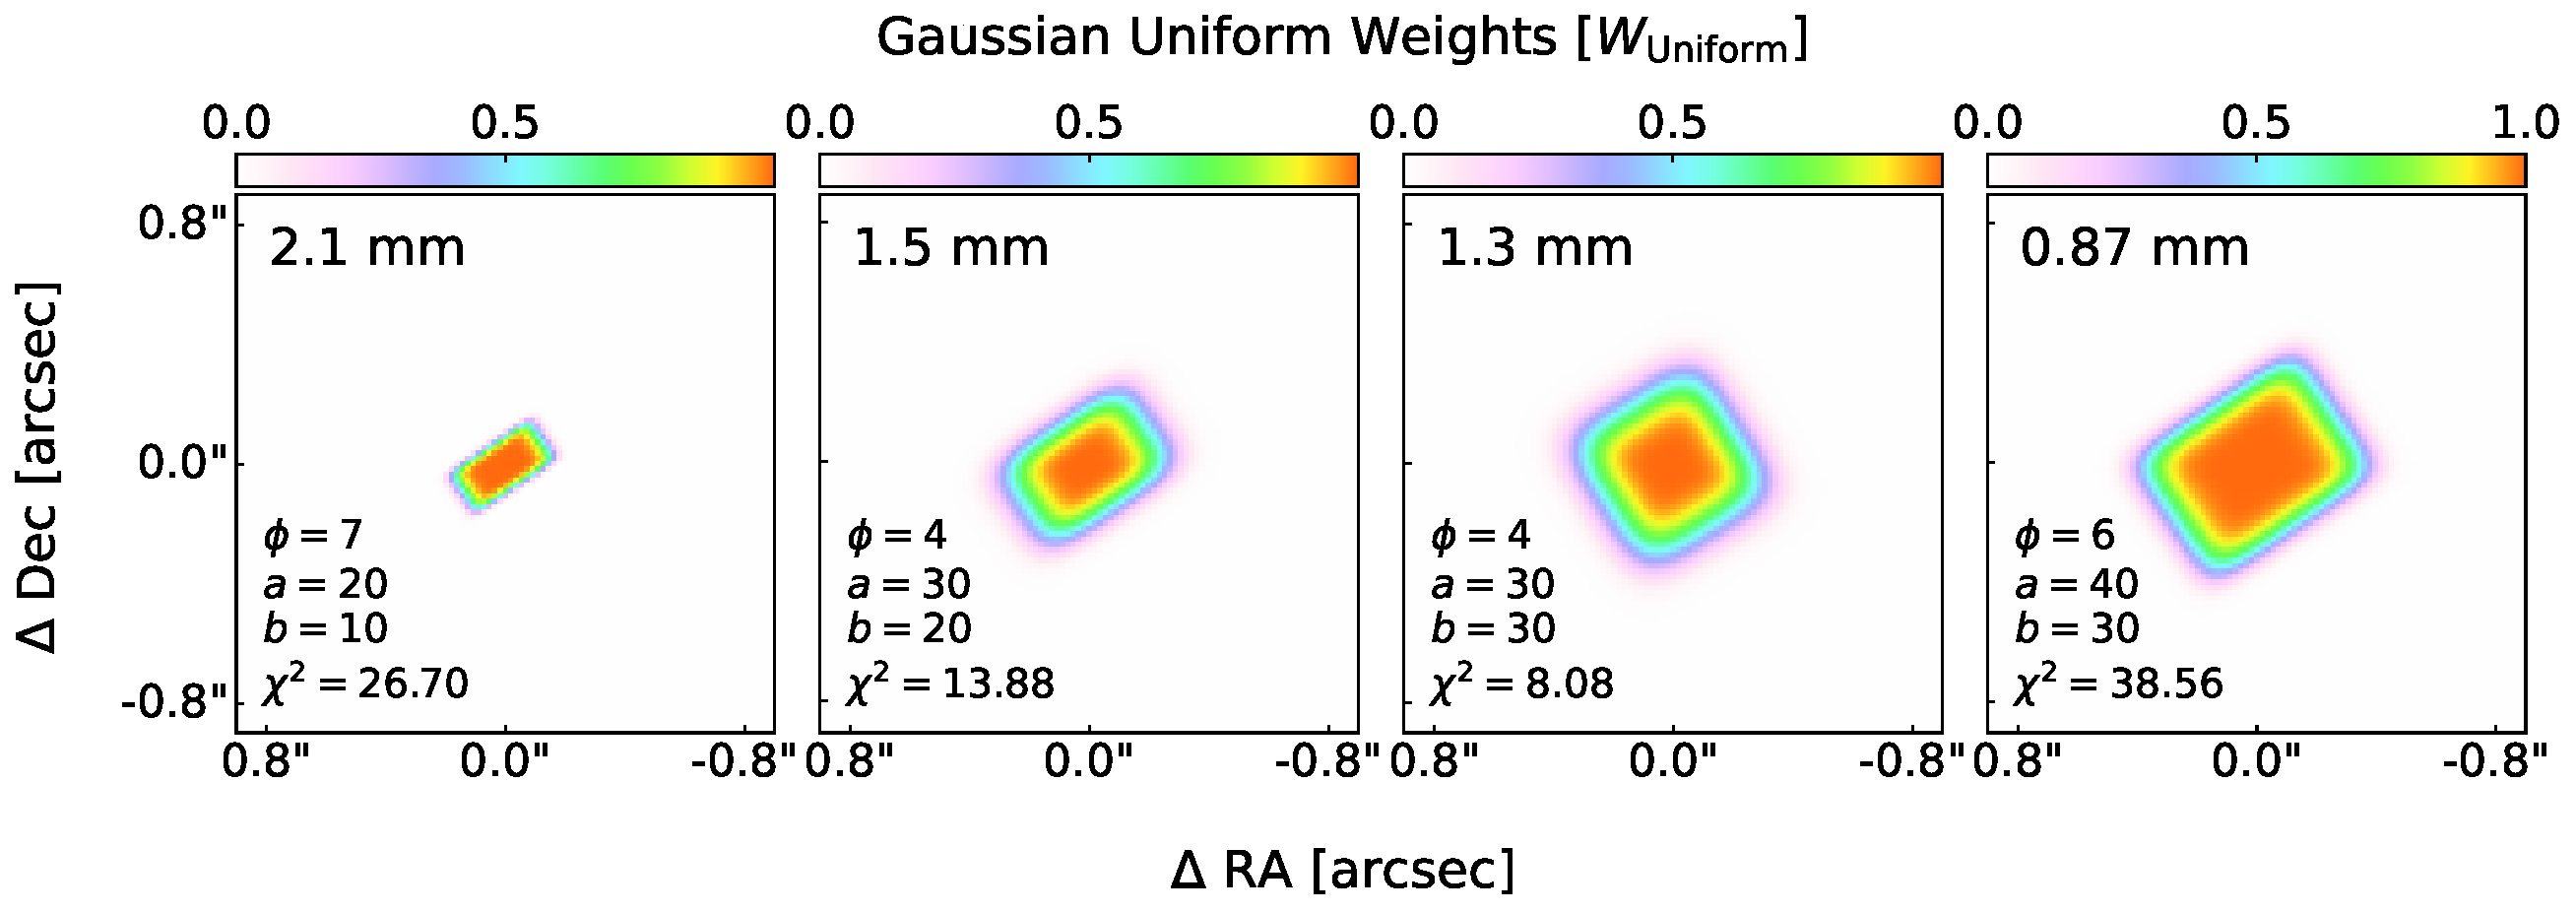
\includegraphics[width=0.99\textwidth]{WRITEUP_AND_IMAGES/IMAGES/WRITEUP/Gaussian/Best_grid_Delta_map.pdf}
  \caption[Maps of the Gaussian uniform weights for the best-fit Gaussian model.]{Maps of the Gaussian uniform weights $W_{\text{uniform}}$ (Equation \ref{eq: gaussian_eq}) for the best-fit Gaussian model for each wavelength, corresponding vector pattern shown in Figure \ref{fig: GaussianBestGrid}. }
  \label{fig: gaussian_best_map_w_uniform}
\end{figure}



The increasing area of the uniform polarization region at shorter wavelengths indicates that the uniform alignment contributes more strongly at shorter wavelengths. This is consistent with what the polarization morphologies shown in Chapter \ref{sec: c4_polarization_maps} and the results from the ratio model suggest. 


The parameter $\Phi$ controls the flatness of the Gaussian, the higher the $\Phi$ value the flatter the Gaussian, transitioning from uniform to azimuthal morphology faster (see Figure \ref{fig: Methods/GaussianExamples}). In the best-fit model at each wavelength, $\Phi$ is greater than 2, producing a flat-topped Gaussian rather than a standard Gaussian. The flattened profiles are also visible in Figure \ref{fig: gaussian_best_map_w_uniform}, since the profile for the uniform weighting shows sharp edges and is more square-shape than round.



% ------------------------------------------------------------------
\subsection{Comparison of Geometric Models}
The \chired values and visual comparisons of the ratio and Gaussian models show that the Gaussian model provides a better overall fit. Figure \ref{fig: RatioBestGrid} shows that, while the ratio model matches many of the observed vectors at each wavelength, it is a poor match for others. This is a limitation of applying the same polarization pattern across the whole disk. As discussed above, the polarization pattern changes with distance from the centre of the disk. Therefore, while the ratio model provides a good first test, it is an oversimplification to accurately model the pattern throughout the entire disk. 


Figure \ref{fig: GaussianBestGrid} shows that, although not all vectors match perfectly, many are accurately reproduced by the Gaussian model. At \bsix and \bsevenNS, the model does not match the vectors along the lobes, which could be related to depolarization. Additionally, as mentioned earlier, the assumed polarization fraction of 2\% could simultaneously overestimate the uniform polarization fractions and underestimate the azimuthal polarization fractions, biasing the model to favour the uniform pattern. Overall, the Gaussian model is the better model but still has limitations, as it is only geometric. 
% ------------------------------------------------------------------